\documentclass[12pt]{report}

\usepackage{amsmath}
\usepackage{pgfplots}
\usepgfplotslibrary{units}
\usepackage[russian]{babel}
\usepackage{filecontents}
\usepackage{titlesec, blindtext, color}
\usepackage{listings}
\usepackage{pdfpages}

\usepackage{titlesec, blindtext, color} 
\definecolor{gray75}{gray}{0.75} 
\newcommand{\hsp}{\hspace{20pt}} 

\usepackage{geometry}
\geometry{top=0.5cm}

\usepackage{float}

\lstset{
	language=C++,
	numbers=left,
	breaklines=true, 
	frame=single,
	texcl=true,
	basicstyle=\ttfamily,
	extendedchars=\true
}

\titleformat{\chapter}[hang]{\Huge\bfseries}{\thechapter\hsp\textcolor{gray75}{|}\hsp}{0pt}{\Huge\bfseries}

\begin{document}
	
	\begin{titlepage}
		\centering
		{\scshape\LARGE МГТУ им. Баумана \par}
		\vspace{3cm}
		{\scshape\Large Лабораторная работа №7\par}
		\vspace{0.5cm}	
		{\scshape\Large По курсу: "Анализ алгоритмов"\par}
		\vspace{1.5cm}
		{\huge\bfseries Поиск подстроки в строке\par}
		\vspace{2cm}
		\Large Работу выполнил: Подвашецкий Дмитрий, ИУ7-54Б\par
		\vspace{0.5cm}
		\LargeПреподаватели:  Волкова Л.Л., Строганов Ю.В.\par
		
		\vfill
		\large \textit {Москва, 2019} \par
	\end{titlepage}
	
	\tableofcontents


	\chapter{Аналитическая часть}
	\section{Цели и задачи работы}


Цель лабораторной работы: изучить алгоритмы поиска подстроки в строке. \\*
В рамках выполнения работы необходимо решить следующие задачи:
\begin{itemize}
	\item изучить стандартный алгоритм, алгоритмы Кнута-Морриса-Пратта и Бойера-Мура;
	\item реализовать данные алгоритмы;
	\item привести подробное описание работы каждого алгоритма.
\end{itemize}


	\section{Описание алгоритмов}


\textbf{Постановка задачи:} пусть даны строки \textit{source} и \textit{pattern}, обозначим их \textit{s} и \textit{p} соответственно.  
Необходимо проверить входит ли строка \textit{p} в \textit{s}, если да, то найти индекс первого вхождения.

\subsection{Стандартный алгоритм}
Стандартный алгоритм основан на последовательном сравнении всех подстрок строки \textit{s} с \textit{p}, т.е. будет происходить сравнение всех подстрок размера $|p|$, начиная с индексов $i = 1,2,...,|s|-|p|+1$.

Пусть $s= "abcabccba"$, $p = "cab"$. В таблце 1 показаны сравнения символов, выполняемые в ходе работы алгоритма.
\begin{table}[h]
	\caption{Таблица коэффициентов для класса данных №1}
	\begin{center}
		\begin{tabular}{|c|c|c|c|c|c|c|c|c|c|}
			\hline
			№&a&b&c&a&b&c&c&b&a\\
			\hline	    			
			1&c&a&b& & & & & &\\
			\hline	    			
			2& &c&a&b& & & & &\\
			\hline	    			
			3& & &c&a&b& & & &\\
			\hline	    			
		\end{tabular}
		\label{T:t1}	
	\end{center}
\end{table}

\textbf{Поэтапное описание алгоритма:}
\begin{enumerate}
	\item $i = j = 0$, $i \in [0, |s|-1], j \in [0, |p| - 1]$.
	\item Посимвольно сравниваем \textit{s} c \textit{p}, \textit{s[i]} c \textit{p[j]}.
	\item Если найдено совпадение, то увеличиваем $i$ и $j$, если $j=|p|$, то подстрока найдена, иначе прикладываем \textit{p} к следующему символу \textit{s}.
\end{enumerate}

В листинге 1 представлена реализация стандартного алгоритма.
\begin{lstlisting}[frame=single,caption=Стандартный алгоритм, breaklines]
int standart(const std::string &str, const std::string &substr)
{
	const size_t str_len = str.length();
	const size_t sub_len = substr.length();
	
	for (size_t i = 0; i <= str_len - sub_len; i++)
	{
		size_t tmp = i;
		
		for (size_t j = 0; j < sub_len; j++)
		{
			if (substr[j] != str[tmp])
			{
				break;
			}
			
			if (j == sub_len - 1)
			{
				return static_cast<int>(i);
			}
			
			tmp++;
		}
	}
	
	return -1;
}
\end{lstlisting}

\subsection{Алгоритм Кнута-Морриса-Пратта}

Алгоритм Кнута-Морриса-Пратта является оптимизацией стандартного алгоритма. Необходимо дать определения префикса, суффикса и префикс-функции.

Префикс \textit{pf} строки \textit{s} - последовательность символов строки такая, что $pf=s[0,...,i), i \in [0, |s|-1]$.

Суффикс \textit{sf} строки \textit{s} - последовательность символов строки такая, что $sf=s[i,...,|s|-1], i \in [1, |s|-1]$.

Префикс-функция строки \textit{s} на позиции \textit{i} - функция, возвращающая длину \textit{k} наибольшего собственного префикса строки \textit{s}, совпадающего с суффиксом этой строки.

Пусть строка $s = "cbcbc"$, рассмотрим все ее суффиксы, префиксы и значения префикс-функции, представленные в таблице 2.

\begin{table}[h]
	\caption{Пример таблицы префиксов и суффиксов для строки s}
	\begin{center}
		\begin{tabular}{|c|c|c|c|}
			\hline
			i&Prefix(s,i)&префиксы&суффиксы\\
			0&0&c&\_\\
			1&0&c&b\\
			2&1&c, cb&c, bc\\
			3&3&c, cb, cbc&c, bc, cbc\\
			4&3&c, cb, cbc, cbcb&c, bc, cbc, bcbc\\
			\hline
		\end{tabular}
		\label{T:t1}	
	\end{center}
\end{table}

Данный алгоритм использует автомат, прикладывание искомой подстроки к строке происходит при помощи вспомогательного массива сдвигов.

Алгоритм заполнения массива сдвигов:
\begin{enumerate}
	\item Создать массив $shift, |shift| = |p|$;
	\item $shift|0| = 0$;
	\item $i=1,j=0$ -- индексы для строки и массива сдвигов соответственно;
	\item Сравниваем $p[i]$ и $p[j]$, при совпадении $shift[i] = j+1$, сдвигаемся на символ вперед; иначе если $j = 0$, длина префикса нулевая, то $shift[i] = 0$.
	\item Если $j \neq 0$, то $j = shift[j-1]$.
	\item Если просмотрена не вся строка, то возвращаемся на 4ый шаг.
\end{enumerate}

Шаблонная строка устанавливается в начало исходной, затем аналогично стандартному алгоритму проводтся посимвольное сравнение. При нахождении несоответствия выполняется сдвиг \textit{p} с помощью массива сдвигов. Таким образом удается снизить число сравнений.

Рассмотрим работу алгоритма на примере $s = "abacababda, p = "abab"$, см. рис. 1.
\begin{figure}[H]	
	{
		\centering
		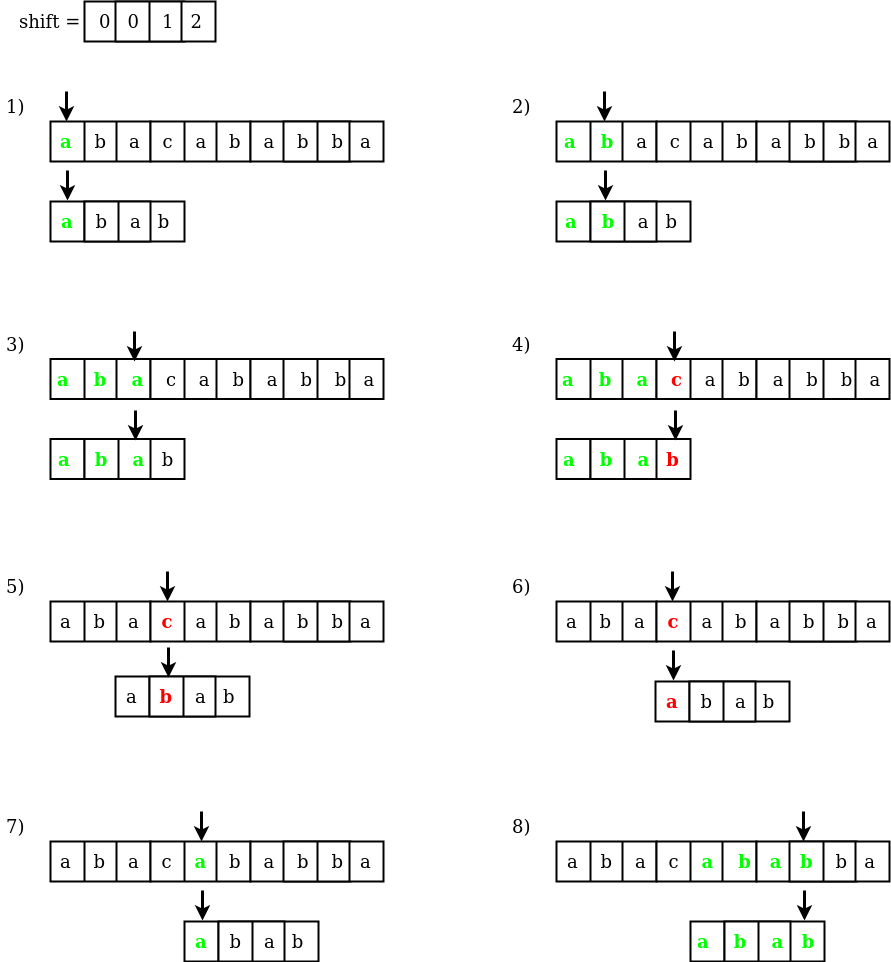
\includegraphics[scale=0.40]{1.png}
		\caption{Пример работы алгоритма Кнута-Морриса-Пратта.}
		\label{pic:ant_schema}
	}
\end{figure}

В листинге 2 представлена реализации алгоритма Кнута-Морриса-Пратта.
\begin{lstlisting}[frame=single,caption=Алгоритм Кнута-Морриса-Пратта, breaklines]
int kmp(std::string &str, std::string &substr)
{
	auto str_len = str.length();
	auto sub_len = substr.length();
	
	if (str_len < sub_len) {
		return -1;
	}
	
	std::vector<size_t> shift(sub_len);
	shift[0] = 0;
	
	for (size_t i = 1; i < sub_len; i++) {
		size_t j = shift[i - 1];
		while (j > 0 && substr[i] != substr[j]) {
			j = shift[j - 1];
		}
		if (substr[i] == substr[j]) {
			j++;
		}
		shift[i] = j;
	}
	
	for (size_t j = 0, i = 0; i < str_len; i++) {
		while (j > 0 && str[i] != substr[j]) {
			j = shift[j - 1];
		}
		if (str[i] == substr[j]) {
			j++;
		}
		if (j == sub_len) {
			return static_cast<int>(i - j + 1);
		}
	}
	
	return -1;
}
\end{lstlisting}

\subsection{Алгоритм Бойера-Мура}

Рассмотрим пошагово алгоритм Бойера-Мура:
\begin{enumerate}
	\item Построить таблицу смещений для каждого символа.
	\item Совмещение \textit{s} и \textit{p} по началу.
	\item Сравнение символов справа налево. Если найдено несовпадение, то \textit{p} смещается вправо на число символов, взятое из таблицы смещений по символу исходной строки, иначе переходим к следующему символу.
	\item Если просмотрена не вся исходная строка, то переход к пункту 3.
\end{enumerate}

Отдельно рассмотрим построение таблицы смещений. Необходимо построить ее так, чтобы пропустить максимально возможное количество незначащих символов. Для этого каждому символу ставится в соответствие величина, равная разности длины шаблона и порядкового номера символа (если символ повторяется, то берется самое правое вхождение, при этом последний символ не учитывается), что равносильно порядковому номеру символа, если считать его с конца строки. Это дает возможность смещаться вправо на максимальное число позиций.

На рис. 2 приведен пример генерации таблицы смещений символов для $s = "cbcbc"$.

\begin{figure}[H]	
	{
		\centering
		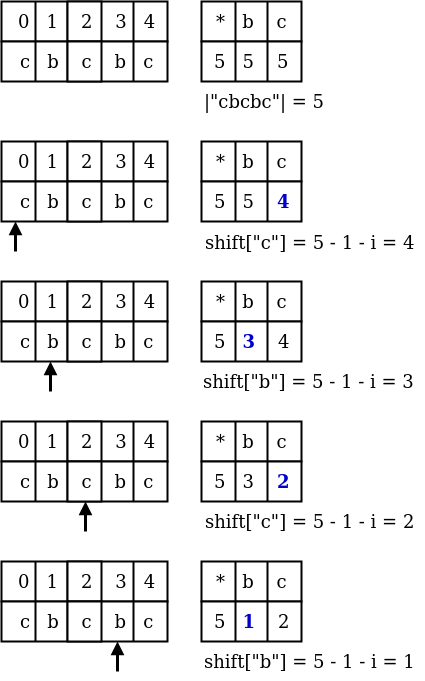
\includegraphics[scale=0.40]{2.png}
		\caption{Пример генерации таблицы сдвигов.}
		\label{pic:ant_schema}
	}
\end{figure}


На рис.3 приведен пример работы алгоритма Бойера-Мура при $s = "abcdefgabc", p = "efg"$.

\begin{figure}[H]	
	{
		\centering
		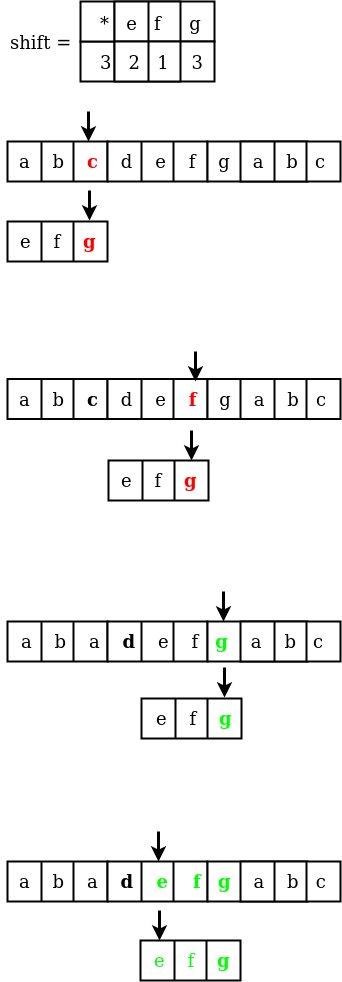
\includegraphics[scale=0.40]{3.png}
		\caption{Пример работы алгоритма Бойера-Мура.}
		\label{pic:ant_schema}
	}
\end{figure}
На листинге 3 представлена реализация алгоритма Бойера-Мура.
\begin{lstlisting}[frame=single,caption=Стандартный алгоритм, breaklines]
std::map<char, size_t> get_shift(const std::string &substr) {
	size_t alphabet_size = 256;
	auto sub_size = substr.length();
	std::map<char, size_t> shift;
	
	for (size_t symb = 0; symb < alphabet_size; ++symb) {
		shift[static_cast<char>(symb)] = sub_size;
	}
	
	for (size_t symb = 0; symb < sub_size - 1; ++symb) {
		shift[static_cast<char>(substr[symb])] = sub_size - symb - 1;
	}
	
	return shift;
}

int bm(std::string &str, std::string &substr) {
	auto str_len = str.length();
	auto sub_len = substr.length();
	if (str_len < sub_len) {
		return -1;
	}
	
	auto shift = get_shift(substr);
	auto start = sub_len - 1;
	auto i = start;
	auto j = start;
	auto k = start;
	
	while (j >= 0 && i < str_len) {
		j = start;
		k = i;
	while (j >= 0 && str[k] == substr[j]) {
		--k;
		--j;
	}
	
		i += shift[str[i]];
	}
	
	return static_cast<int>(k >= str_len - sub_len ? -1 : k + 1);
}

\end{lstlisting}
\begin{center}
	\section*{Вывод}
	\addcontentsline{toc}{section}{Вывод}
\end{center}	
По итогам аналитического раздела были описаны стандартный алгоритм, алгоритм Кнута-Морриса-Пратта и алгоритм Бойера-Мура для нахождения подстроки в строке.



\begin{center}
	\chapter*{Заключение}
	\addcontentsline{toc}{chapter}{Заключение}
\end{center}
\label{sec:ending}


Таким образом, в ходе лабораторной работы были изучены, описаны и реализованы стандартный алгоритм, алгоритм Кнута-Морриса-Пратта и алгоритм Бойера-Мура для нахождения подстроки в строке. 

\end{document}
